Tässä luvussa esitetään perusteet ja tarvittavat tiedot ohjelmistojen testauksesta ja testiautomaatiosta, jotka liittyvät työn laajempaan teoreettiseen kehykseen.
Ensin esitetään testiautomaation tarkoitus, jonka jälkeen käydään yksityiskohtaisesti läpi ohjelmistotestauksen tasot ja niiden merkitystä testiautomaatiossa.
Ohjelmistojen testaukseen ja erityisesti testiautomaatioon sekä tämän diplomityön aiheeseen liittyvät käsitteet testitapaus ja testikokoelma esitetään omassa kappaleessaan.
Lopuksi vielä esitetään tarvittavia jatkuvan integroinnin ja testausvetoisen kehityksen perusteita sekä pyritään luomaan lukijalle ymmärrystä siitä, miten ne liittyvät niitä laajempaan testiautomaation käsitteeseen ja diplomityön tuloksien käyttöönottoon.

Testiautomaation perusteiden ymmärtämistä tarvitaan varsinkin työn myöhemmissä vaiheissa, joissa esitetään testiautomaatioon liittyvien hyväksymistestauksen testitapauksien testausjärjestelmä ja tutkimusongelmaan vastaava varsinainen priorisointi painotetun verkon avulla.

\section{Testiautomaation tarkoitus} \label{ch:07_testiautomaation_tarkoitus}

  Testiautomaation tarkoitus on pohjimmiltaan mahdollistaa ohjelmistotuotteen jatkuva, tehokas ja vaivaton laadunvarmistus nyt ja tulevaisuudessa.
  Testiautomaation vastakohtana voidaan ajatella manuaalista testausta, joka vaatii täydellistä ihmisen vuorovaikutusta testauksen suorittamiseen.
  Testiautomaatiossa käytetään erityisiä ohjelmistotyökaluja ennalta määritettyjen testitapauksien suorittamiseen, ihmisen tekemän manuaalisen testauksen sijaan.
  Ohjelmistojen testaamisella itsessään pyritään löytämään ohjelmistotuotteesta virheitä ja anomalioita sekä varmistamaan, että se toimii asetettujen vaatimusten sekä suunnitelmien mukaisesti.
  Testauksen automatisoiminen vapauttaa aikaa, kustannuksia ja henkilöresursseja manuaalisesta testaamisesta muihin tuotantotehtäviin sekä parantaa toistettavien testien luotettavuutta poistamalla manuaalisessa testauksessa tapahtuvat inhimillisen virheet.
  Testiautomaatiolla, joka kytketään osaksi ohjelmistotuotantoprosessia, voidaan myös löytää ohjelmistokehityksen aikana ohjelmistokoodiin lipsuvia virheitä ja näin ollen saavuttaa mahdollisuus korjata niitä ennen kuin ohjelmisto julkaistaan loppukäyttäjille.

  Laadunvarmistuksen osalta ohjelmistokehityksessä on usein käytetty niin sanottuja laadullisia ominaisuuksia, joiden kattamisella voidaan validoida laatua.
  Laadullisia ominaisuuksia ovat ISO 9126-standardin mukaan \parencite{iso_9126-1_2001}:

  \begin{itemize}
    \item toiminnallisuus
    \item luotettavuus
    \item käytettävyys
    \item tehokkuus
    \item ylläpidettävyys
    \item siirrettävyys
  \end{itemize}

  Näistä laadullisista ominaisuuksista testiautomaatiolla pystytään kattamaan erityisesti toiminnallisia, luetettavuudellisia ja tehokkuudellisia ominaisuuksia.
  Käytettävyyden, ylläpidettävyyden ja siirrettävyyden validointi puolestaan on vaikeampaa testiautomaation avulla, sillä ne ovat varsin subjektiivisia.
  Tässä diplomityössä testiautomaation yhteydessä keskitytään hyväksymistestauksen kannalta erityisesti toiminnallisiin laatuominaisuuksiin ja niiden testaamiseen.

\section{Testauksen tasot} \label{ch:07_testauksen_tasot}

  Testauksen tasoja on useita ja usein ohjelmistojen kattavaan testaamiseen on suositeltavaa käyttää ohjelmistotuotantoprosessissa eri tasojen yhdistelmää.
  Ohjelmistojen testaus usein jaotellaan kolmeen erilaiseen menetelmään, jotka myös vaikuttavat eri testauksen tasojen käyttökelpoisuuteen.
  Erilaisia menetelmiä ovat mustalaatikkotestaus, harmaalaatikkotestaus ja valkolaatikkotestaus, jotka eroavat toisistaan yleisesti ottaen siinä, otetaanko tieto ohjelmistotuotteen sisäisestä toteutuksesta mukaan itse testaamiseen.
  Testauksen tasot esitetään kirjallisuudessa usein hieman eri muodoissa, mutta yleisesti ne jaetaan neljään eri tasoon, jotka voidaan kuvata pyramidin tasoavaruuteen projisoituna muotona.

  \begin{figure}[H]
    \centering
    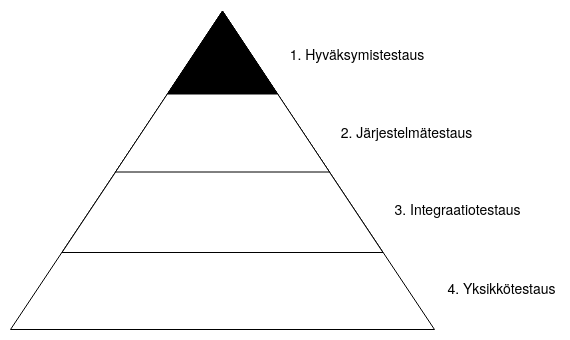
\includegraphics[width=0.8\textwidth]{assets/testauksen-tasot.png}
    \caption{Testauksen tasot pyramidin muodossa}
    \label{fig:testing-levels-pyramid}
  \end{figure}

  Pyramidimuodossa esitetyistä testauksen tasoista kaikkiin on mahdollista soveltaa testiautomaatiota.
  Testauksen menetelmien osalta hieman yksinkertaistaen valkolaatikkotestauksen alaisuuteen kuuluvat yksikkötestaus ja integraatiotestaus sekä mustalaatikkotestauksen alaisuuteen kuuluvat järjestelmätestaus ja hyväksyntätestaus.
  Pyramidimuodossa alimpana kuvataan aina yksikkötestaus, joka on tasoista atomisin ja myös luo vahvan pohjan kokonaisvaltaiselle testaamiselle.
  Noustessa pyramidissa ylöspäin, atomisuus häviää ja testattavana olevan kohteen laajuus sekä kompleksisuus kasvavat.
  Ylimpänä pyramidissa on hyväksymistestaus, joka on tarkoituksellista toteuttaa vaatimusmäärittelyn täyttävää valmista järjestelmää vastaan siten, että sen varmistetaan vastaavan loppukäyttäjän tarpeita.
  Monissa tapauksissa järjestelmätestauksen ja hyväksymistestauksen rajat saattavat olla epäselvät ja häilyvät.
  Tässä työssä hyväksymistestauksella tarkoitetaan käyttäjän hyväksyttämistestausta (UAT), jotta järjestelmätestauksen ja hyväksymistestauksen väliset eroavaisuudet tulevat lukijalle selkeästi esille.

  Hyväksymistestaus on tämän diplomityön keskiössä ja siihen liittyvää teoriaa esitetään vielä laajemmin omassa hyväksymistestaus luvussaan \ref{ch:08_hyvaksymistestaus}.
  Seuraavissa kappaleissa esitetään vielä yksityiskohtaisemmin jokainen pyramidissa \ref{fig:testing-levels-pyramid} esitetty testauksen taso, jotta lukijalle muodostuisi käsitys erityisesti hyväksymistestauksen suhteesta muihin testauksen tasoihin.

  \subsection{Yksikkötestaus} \label{ch:07_yksikkotestaus}

    Yksikkötestauksen ajatuksena on testata ohjelmistotuotteen lähdekoodista löytyviä yksiköitä, kuten luokkia, funktioita tai moduuleita.
    Yksikkötestaus toteutetaan ohjelmiston toteuttavia pienimpiä yksikköjä vastaan ja sen avulla pyritään validoimaan, että jokainen yksikkö toimii siten kuin ne on ohjelmistokehityksen aloitusvaiheessa suunniteltu toimimaan.
    Yksikkötestaus eroaa muista testauksen tasoista siinä, että sen voi suorittaa ainoastaan ohjelmistokehittäjät tai muut ohjelmiston lähdekoodiin perehtyneet henkilöt.
    Yksikkötestaus on näin ollen teknisesti valkolaatikkotestausta.
    Yksikkötestausta tarvitaan, jotta voidaan pyrkiä varmistamaan, että ohjelmiston koostavat pienimmät yksiköt toimivat tarkoituksenmukaisella tavalla.

    Yksikkötestauksen toteuttamiseen käytetään pääsääntöisesti jotakin tarkoitusta varten räätälöityä testikirjastoa, joissa on keskenään yleensä hyvin samankaltainen perusperiaate.
    Yksikkötestaukseen tarkoitetuissa testikirjastoissa löytyy usein yksittäisen testitapauksen kuvaava tietorakenne, esimerkiksi luokka, sekä siihen usein kuuluvat alustus- ja lopetusfunktiot.
    Näiden lisäksi varsinainen testauskoodi toteutetaan pääsääntöisesti käyttäen niin sanottuja testikirjaston tarjoamia assert-funktioita, joiden avulla voidaan esimerkiksi varmistaa, onko jokin muuttuja tietyssä arvossa.

    Yksikkötestausta hyödynnetään usein myös ketterien menetelmien aihepiirissä, jossa ohjelmistotuotantoa voidaan toteuttaa muun muassa niin sanotulla testausvetoisella kehityksellä \ref{ch:07_testausvetoinen_kehitys}.
    Testausvetoisessa kehityksessä yksikkötestauksen osalta, ohjelmistokehittäjät laativat ensisijaisesti yksiköiden yksikkötestit ennen niiden toteuttamisen aloittamista.

    Ohjelmistotestauksen tasojen pyramidissa ja hyvin toteutetussa ohjelmistotestauksen monitasoisessa testauksessa tämä testauksen taso on usein testitapauksien määrässä kaikista laajin.
    Monitasoisessa testauksessa yksikkötestaus luo tärkeän pohjan testaamiselle kokonaisuutena ja antaa tietoa ohjelmiston pienimpien yksiköiden toimivuudesta.
    Yksikkötestaus on myös paljon käytetty ja tärkeä osa testiautomaatiossa, sillä se varmistaa sovelluksen yksiköiden suunniteltua toimintaa.

  \subsection{Integraatiotestaus} \label{ch:07_integraatiotestaus}

    Integraatiotestauksen ajatuksena on testata ohjelmistotuotteen toteuttavien eri komponenttien yhteensopivuutta niiden rajapintojen osalta.
    Integraatiotestaus toteutetaan ohjelmiston suunnitelmaa ja suunniteltua mallia vastaan.
    Integraatiotestauksen onnistunut toteuttaminen luo validoitavan perustan ohjelmiston toimimiseen ja sen koostamiseen kokonaisena, eri komponenteista koostuvana järjestelmänä.
    Integraatiotestausta tarvitaan, jotta voidaan varmistaa sovelluksen yksiköiden yhteensopivuus, joka ei pelkällä yksikkötestauksella tulisi muuten katetuksi.

    Integraatiotestauksen kohteita voivat olla esimerkiksi luokkien ja moduulien väliset rajapinnat sekä web-sovelluksien api-ohjelmointirajapinnat.
    Integraatiotestauksen toteutuksen kannalta voidaan usein käyttää myös yksikkötestaukseen tarkoitettuja testikirjastoja ja työkaluja, mutta itse testitapauksien rakenne on silloin yksikkötestauksen testitapauksista merkittävällä tavalla erilainen.
    Integraatiotestauksessa testitapauksien rakenteeseen tulee assert-funktioiden lisäksi myös usein tarvetta jäljitellä rajapintojen tarjoamaa dataa.
    Rajapintojen tarjoaman datan jäljittelemiseen on olemassa useita valmiita työkaluja ja kirjastoja, joita integraatiotestauksen tapauksessa voi käyttää testitapauksien rakentamisen apuna.

    Integraatiotestauksen yhteydessä puhutaan usein myös niin sanotusta savutestauksesta, jonka tarkoituksena integraatiotestauksen yhteydessä on koostaa toistuva, esimerkiksi päivittäinen, koontiversio ohjelmistosta ja testata sen kriittisten komponenttien yhteensopivuus.
    Integraatiotestaus on myös tärkeä osa testiautomaatiota, sillä sen avulla voidaan varmistaa sovelluksen yksiköiden, kuten esimerkiksi luokkien, komponenttien tai moduulien yhteensopivuus.

  \subsection{Järjestelmätestaus} \label{ch:07_jarjestelmatestaus}

    Järjestelmätestauksen ajatuksena on testata kokonaista ja toimivaa järjestelmää, yhtenä suurena yksikkönä.
    Järjestelmätestausta tarvitaan, jotta voidaan varmistaa kokonaisen ohjelmiston toimivuus, jota ei muuten pelkällä yksikkötestauksella ja integraatiotestauksella saataisi täydellisellä varmuudella selville.

    Järjestelmätestaukseen liittyy laajasti erilaisia testattavia laadullisia ominaisuuksia kuten toiminnallisuus, luotettavuus, käytettävyys, tehokkuus, ylläpidettävyys ja siirrettävyys \parencite{iso_9126-1_2001}.
    Aiemmin testiautomaation tarkoitus kappaleessa \ref{ch:07_testiautomaation_tarkoitus} esitettiin että, edellä mainituista laadullisista ominaisuuksista kaikki eivät sovellu hyvin testiautomaation avulla testattaviksi.
    Esitetyistä syistä johtuen, automatisoidulla järjestelmätestauksella voidaan testata edellä mainituista ominaisuuksista lähinnä ohjelmiston toiminnallisuutta, luotettavuutta ja tehokkuutta.
    Toiminnallisuutta voidaan testata käyttöliittymätestauksella, joka on mahdollista automatisoida käyttötapauksien muotoon.
    Luotettavuutta voidaan testata automaattisesti tietoturvaa testaavien käyttötapauksien muodossa.
    Tehokkuutta voidaan testata automaattisesti lisäämällä aikaleimoihin perustuvaa tarkastelua testitapauksiin, sekä tehdä kuormitusta testaavia testitapauksia.
    Edellä mainituista muista laadullisista ominaisuuksista voidaan toki kuitenkin ylläpidettävyyttä ja siirrettävyyttä testata manuaalisesti.


    Testauksen tasona järjestelmätestaus voi olla testiautomaation teknisen toteutuksen kannalta jopa hyvin samanlainen kuin sitä spesifimpi hyväksymistestaus.
    Usein kuitenkin hyväksymistestauksessa paneudutaan erityisesti vaatimusmäärittelyyn ja asiakaslähtöiseen testaamiseen, kun taas järjestelmätestauksessa voidaan testata esimerkiksi myös järjestelmän tehokkuutta tai tietoturvaa.
    Tämä on tosin täysin riippuvainen vaatimusmäärittelystä, joten jos tehokkuus ja tietoturva ovat ohjelmiston asiakasvaatimuksia niin niiltä osin järjestelmätestaus ja hyväksymistestaus lomittuvat.
    Joissakin yhteyksissä järjestelmätestaus ja hyväksymistestaus esitetään jopa yhteisenä testauksen tasona, etenkin silloin kun testiautomaation kannalta ne esimerkiksi edellä mainitulla tavalla muistuttavat kovasti toisiaan.
    Järjestelmätestaus osittain hyväksymistestauksen kanssa on erittäin merkittävä osa testiautomaatiosta, sillä sen avulla voidaan testata toteutettavaa järjestelmää kokonaisuutena.

  \subsection{Hyväksymistestaus} \label{ch:07_hyvaksymistestaus}

    Hyväksymistestauksen ajatuksena on varmistaa toteutettavan ohjelmiston vaatimusten toimivuus erityisesti käytännön tilanteissa siten, että voidaan varmistaa vastaako ohjelmisto loppukäyttäjän tarpeita.
    Hyväksymistestaus toteutetaan ohjelmiston toimintoja kuvaavaa vaatimusmäärittelyä tai loppukäyttäjistä sekä heidän tarpeista laadittuja käyttötapauksia vastaan.
    Hyväksymistestauksen rooli testiautomaatiossa ja erityisesti jatkuvan integraation yhteydessä on osoittaa, voidaanko järjestelmä sellaisenaan julkaista loppukäyttäjille.

    Hyväksymistestaus testaa lähinnä toiminnallisia laatuominaisuuksia ja usein se toteutetaan käyttöliittymätasolla testitapauksien muodossa.
    Poikkeuksena toiminnallisien ominaisuuksien lisäksi hyväksymistestauksessa voi olla mukana muita laadullisia ominaisuuksia vain jos ne ovat asiakastarpeiden mukaisia, joka on kuitenkin tavallisesta varsin poikkeava tilanne.
    Samassa asiayhteydessä puhutaan usein myös niin sanotusta e2e-testauksesta, eli päästä päähän -testauksesta.
    Päästä päähän -testauksessa on tarkoituksena toteuttaa testaaminen siten, että testaus pitää sisällään kaiken siltä väliltä mitä loppukäyttäjä voi tarpeidensa saavuttamiseksi tehdä ja nähdä aloittaessaan ohjelmiston käytön ja lopettaessaan sen käytön.

    Testiautomaatio on äärimmäisen hyödyllinen hyväksymistestauksen osalla, koska sillä voidaan automatisoida ohjelmiston validointi ja hyväksyminen, sekä parhaimmillaan estää puutteellisesti toimivan ohjelmiston julkaiseminen.
    Hyväksymistestausta tarvitaan myös, jotta voidaan testata ja validoida vaatimusten ja loppukäyttäjän tarpeiden mukaisten ominaisuuksien toimivuus kokonaisessa järjestelmässä.

\section{Testitapaus ja testikokoelmat} \label{ch:07_testitapaus_ja_testikokoelmat}

  Testitapaus on ohjelmistotestauksen automatisoimisen kannalta erittäin tärkeä käsite.
  Testitapaus kuvaa yhden testattavana olevan asian testaamiseksi suoritettavaa tai suoritettavia toimenpiteitä.
  Testitapauksen sisältämien toimenpiteiden suorittamisen tarkoituksena on saada selville täyttääkö se toimenpiteiden mukaiset ehdot ja toimiiko testattava asia oikein.
  Testitapauksella on usein alustusvaihe, varsinainen testausvaihe ja lopetusvaihe.
  Alustusvaiheessa testitapauksen vaativa ympäristö ja muuttujat alustetaan.
  Varsinaisessa testitapauksen testausvaiheessa suoritetaan testattavan asian testaukseen liittyvät toimenpiteet.
  Lopetusvaiheessa testitapauksen ajaksi muodostettu ympäristö usein tuhotaan ja käytetyt resurssit nollataan, jotta ne eivät enää vaikuta muihin testitapauksiin.

  Testikokoelma on yksittäisistä testitapauksista koostuva ryhmitelty testitapauksien joukko.
  Testikokoelman saattaa kuulua myös sellaisia testitapauksia, joiden suoritusjärjestys on etukäteen määritetty.
  Suoritusjärjestyksellisissä testikokoelmissa voi esiintyä testitapauksia, jotka toimivat samassa testausympäristössä, muokaten ja jättäen jälkiä omasta suorituksestaan.
  Myöhemmin suoritusjärjestyksessä tulevat testitapaukset voivat siinä tapauksessa hyötyä tai vaatia testausympäristön ominaisuuksia, jotka aiemmat testitapaukset ovat asettaneet.
  Testikokoelman sisältämät testitapaukset voidaan kuitenkin luonnollisesti laatia myös sellaisella tavalla, että jokainen testitapaus hoitaa yksityiskohtaiset alustustoimenpiteensä itsenäisesti.

  Testitapauksia voidaan ryhmitellä samaan kontekstiin liittyviksi testikokoelmiksi tilanteesta riippuen monilla eri tavoin.
  Ryhmittelyn perusteen valitsemiseen kannattaa käyttää harkintaa, sillä testikokoelmien laajuus on helpomman hallittavuuden takia tärkeää.
  Yksi tapa ryhmitellä testitapauksia on käyttää ohjelmistojen laadullisia ominaisuuksia ryhmittelyn perustana.
  Tällaisessa ryhmittelyssä yksi kokoelma voi olla toiminnallisille testitapauksille ja toinen tehokkuutta mittaaville testitapauksille.
  Laadullisien ominaisuuksien mukaan tehty testitapauksien ryhmittely saattaa kuitenkin johtaa määrällisesti liian suuriin testitapauksien eroihin testikokoelmien kesken.
  Hyväksymistestauksen näkökulmasta tarkasteltuna testitapauksia on mahdollista ryhmitellä käyttöliittymän näkymiin perustuviin testikokoelmiin.
  Näkymäperusteinen ryhmittely on osaltaan looginen tapa jakaa testitapaukset eri testikokoelmiin, sillä jokainen käyttöliittymän näkymä voidaan tarvittaessa testata erikseen suorittamalla kyseisen testikokoelman testitapaukset.
  Tässä diplomityössä hyödynnetään perustavanlaatuisesti näkymäperusteista testitapauksien ryhmittelyä, koska sen avulla on mahdollista suorittaa testikokoelmien näkymäperusteinen priorisointi työssä myöhemmin esitettävää painotettua verkkoa hyödyntäen.

\section{Jatkuva integrointi} \label{ch:07_jatkuva_integrointi}

  Testiautomaation rakentaminen manuaalisen testaamisen sijaan mahdollistaa sen liittämisen osaksi jatkuvaa integrointia.
  Lisäksi useissa ohjelmistotuotannon prosesseissa pelkkä manuaalinen testaus kävisi selkeästi automatisoitujen koonti- tai julkaisuputkien periaatteita vastaan.
  Testiautomaation tarkoitus kappaleessa \ref{ch:07_testiautomaation_tarkoitus} aiemmin esitettiin testiautomaation ja manuaalisen testauksen eroa hyötyjen ja haittojen näkökulmasta.
  Testiautomaation toteuttaminen testitapauksien muodossa on jo itsessään testiautomaatiota, mutta käsitettä voidaan kuitenkin laajentaa, että myös jatkuva integrointi liittyy oleellisesti testiautomaation toteuttamiseen varsinkin nykyaikana ja erityisesti ketteriin menetelmiin painottuvassa ohjelmistokehityksessä.

  Jatkuvalla integroinnilla tarkoitetaan versiohallintaisessa ohjelmistokehityksessä väistämättömän integrointiprosessin muuntamista luonnostaan jatkuvaksi.
  Ohjelmistokehityksessä integrointiprosessi tulee vastaan, kun eri ohjelmistokehittäjät tai tiimit toteuttavat muutoksia tai uusia ominaisuuksia kehitettävänä olevaan ohjelmistotuotteeseen.
  Tällaisessa tilanteessa yksittäiset ohjelmistokehittäjät tai tiimit toteuttavat uutta ohjelmakoodia toisistaan irrallaan siihen asti, kunnes muutokset tai ominaisuudet tulee yhdistää yhdeksi kokonaiseksi kehityksen kohteena olevaksi ohjelmistotuotteeksi, jota prosessina kutsutaan integrointiprosessiksi.
  Jatkuvan integroinnin tarkoituksena on nopeuttaa integrointiprosessia ja muuttaa ohjelmistokehityksessä käytössä olevia periaatteita siten, että siitä tulee luonnostaan jatkuvaa.
  Jatkuvan integroinnin toteuttaminen tarvitsee teknisesti sen mahdollistavan versionhallintajärjestelmän ja varsinaisen jatkuvan integroinnin palvelimen.

  \begin{figure}[H]
    \centering
    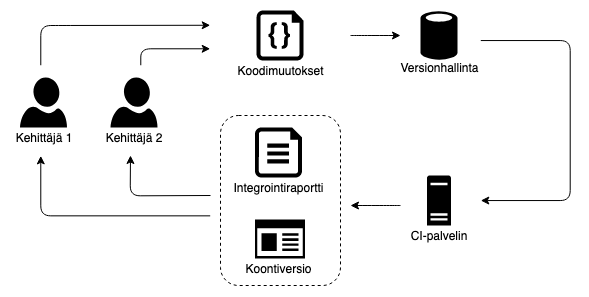
\includegraphics[width=0.8\textwidth]{assets/jatkuva-integrointi.png}
    \caption{Jatkuvan integroinnin perusperiaate on iteratiivinen}
    \label{fig:jatkuva-integrointi}
  \end{figure}

  Esimerkkinä versionhallintajärjestelmänä voidaan käyttää nykyaikana suosittua git-ohjelmistoa ja jatkuvan integroinnin palvelimena esimerkiksi GoCD-ohjelmistoa.
  Perusideana jatkuvassa integroinnissa on konfiguroida jatkuvan integraation mahdollistava palvelinohjelmisto siten, että se kuuntelee versionhallintaan tulevia muutoksia ja suorittaa integrointiprosessin jatkuvasti aina muutoksia huomattuaan.
  Versionhallintaan tulevat muutokset voidaan jatkuvan integraation osalta kuunnella ajastetusti tietyin väliajoin tai aidosti jatkuvalla tavalla käyttämällä esimerkiksi web-koukkuja, jotka tiedottavat jatkuvan integraation palvelimelle versionhallintaan saapuneista muutoksista.
  Jatkuvan integroinnin yhden iteraatiokerran integrointiprosessin tuloksena on tarkoituksena tarjota periaatteeltaan sama lopputulema kuin mitä se olisi manuaalisella integrointiprosessillakin.
  Jatkuvan integroinnin mahdollistava konfiguraatio sisältää aina jonkinlaisen koontiputken tai useita koontiputkia, joissa rakennetaan koontiversio kehitettävän ohjelmiston lähdekoodeista.
  Koontiputki voi sisältää esimerkiksi ohjelman lähdekoodien kääntämisen asiaan sopivalla kääntäjällä.
  Kääntämisen lisäksi koontiputkeen on tässä vaiheessa mahdollista ja erittäin kannattavaa yhdistää testiautomaatiota, kuten esimerkiksi automaattisten yksikkötestien suorittaminen ennen kääntämistä ja hyväksymistestien suorittaminen valmiille koontiversiolle kääntämisen jälkeen.

  Jatkuvan integroinnin yhteydessä suoritettavat testikokoelmat \ref{ch:07_testitapaus_ja_testikokoelmat} ja niiden sisältävät testitapaukset ovat erittäin järkeviä toteuttaa, sillä ne esimerkiksi parantavat ohjelmistokehityksen ja lopputuotteen luotettavuutta ja laatua.
  Jatkuvan integroinnin sisältämästä koontiputkesta saadaan hyödyllistä palautetta ja raportteja integrointiprosessin onnistumisesta, joka voidaan ohjata pääasiassa ohjelmistokehittäjille sekä myös muillekin sidosryhmille.
  Jatkuvalla integroinnilla itsessään on myöskin paljon sen käyttöönoton antamia hyötyjä, kuten esimerkiksi toteutettujen muutosten tai toimintojen integrointitiheyden kasvattamisen tuomat edut.
  Jos muutosten tai toimintojen integroiminen on perinteisessä ohjelmistokehityksessä tehty harvoin, kuten esimerkiksi viikoittain, niin jatkuva integroiminen korjaa sen tuomat haasteet turhan laajasta integrointiprosessista ja mahdollisesta ohjelmistokoodin hajoamisesta.
  Tällaisissa tapauksissa ohjelmakoodi voi sisältää epäyhteensopivia moduuleita tai muita rajapintoja sekä mahdollisuuden käännettävien lähdekoodien kääntämisen onnistumisesta.

\section{Testausvetoinen kehitys} \label{ch:07_testausvetoinen_kehitys}

  Perinteisesti testiautomaatio on soveltunut hyvin vain vakaille ohjelmistoille ja niiden regressiotestaamiseen.
  Nykypäivänä ohjelmistokehitys on siirtynyt suunnitelmapohjaisista prosesseista iteroiviin ketteriin ohjelmistotuotannon prosesseihin.
  Näihin testiautomaatio on soveltunut huonosti, kun testattavaa ohjelmistoa tai lisättyä toiminnallisuutta ei ole vielä olemassa.
  Tähän ongelmaan on kehittynyt niin sanottu testausvetoinen kehitys, jossa testitapaukset suunnitellaan ja toteutetaan ennen varsinaisen ohjelmiston tai toiminnon toteutuksen toteuttamista.

  \begin{figure}[H]
    \centering
    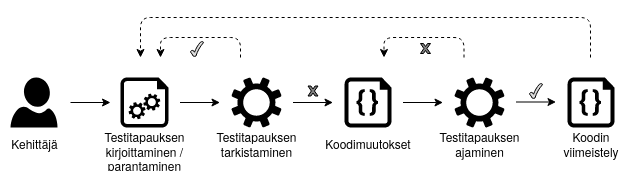
\includegraphics[width=0.8\textwidth]{assets/testausvetoinen-kehitys.png}
    \caption{Testausvetoisen kehityksen vaiheet}
    \label{fig:testausvetoinen-kehitys}
  \end{figure}

  Testausvetoinen kehityksen sisältämät vaiheet \ref{fig:testausvetoinen-kehitys} alkavat testitapauksien luomisesta ja niiden tarkastamisesta.
  Tarkastaminen tapahtuu siten, että testitapaukset suoritetaan sillä oletuksella, että niiden täytyy tässä vaiheessa epäonnistua.
  Alkuvaiheen testitapauksien luomisen jälkeen ohjelmistokehittäjät kehittävät ohjelmistoa tekemällä siihen muutoksia, ihanteellisesti testitapauksien kokoisia paloja kerrallaan.
  Kun koodimuutoksia on syntynyt, riippuen ohjelmistotuotannossa käytössä olevasta integrointiprosessista, ajetaan testitapaukset manuaalisesti tai jatkuvan integroinnin avulla.
  Integrointiprosessista saadaan palautetta, jonka mukaan ohjelmakoodia korjataan tai viimeistellään.
  Testausvetoisella kehityksellä pyritään nopeuttamaan ohjelmistokehitysprosessia verrattuna perinteisiin ohjelmistotuotannon menetelmiin.
  Tämän jälkeen testausvetoista kehitystä käyttävässä ohjelmistotuotantoprosessissa siirrytään takaisin testitapauksien luomiseen ja parantamiseen sekä aloitetaan toinen iteraatiokierros mikäli ohjelmisto ei vielä ole valmis.

  Testausvetoisessa kehityksessä testitapaukset siis laaditaan jo varhaisessa vaiheessa jolloin niiden tekeminen saattaa usein olla liiketoiminnan näkökulmasta helpommin perusteltavaa liiketoiminnan johdolle.
  Tämän lisäksi testitapauksien kirjoittaminen etukäteen luo kattavat testikokoelmat jo alusta alkaen, joita voidaan hyödyntää iteratiivisesti ohjelmistotuotteesta riippuen usein hyvinkin pitkään, etenkin jos niihin tehdään tarvittavaa hienosäätöä ohjelmistokehityksen aikana.
  Ohjelmistokehittäjät voivat kehittää helposti hallittavissa olevia testitapauksien rajaavia kokonaisuuksia, jolloin ohjelmistotuote valmistuu ikään kuin pala kerrallaan.
  Itse ohjelmistokehitys on testausvetoisessa kehityksessä siis iteratiivista ja näin ollen testitapauksien suorittamisesta saadaan palautetta ja raportointia koko ohjelmistotuotantoprosessin aikana.
  Testausvetoinen kehitys kuuluu ohjelmistotuotannossa vahvasti ketterien menetelmien alaisuuteen ja on kasvattanut suosiotaan ketterien menetelmien mukana.
